%%%%%%%%%%%%%%%%%%%%%%%%%%%%%%%%%%%%%%%%%
% Engineering Calculation Paper
% LaTeX Template
% Version 1.0 (20/1/13)
%
% This template has been downloaded from:
% http://www.LaTeXTemplates.com
%
% Original author:
% Dmitry Volynkin (dim_voly@yahoo.com.au)
%
% License:
% CC BY-NC-SA 3.0 (http://creativecommons.org/licenses/by-nc-sa/3.0/)
%
%%%%%%%%%%%%%%%%%%%%%%%%%%%%%%%%%%%%%%%%%

%----------------------------------------------------------------------------------------
%	PACKAGES AND OTHER DOCUMENT CONFIGURATIONS
%----------------------------------------------------------------------------------------

\documentclass[12pt,a4paper]{article} % Use A4 paper with a 12pt font size - different paper sizes will require manual recalculation of page margins and border positions
\usepackage[utf8]{inputenc}
\usepackage{marginnote} % Required for margin notes
\usepackage{wallpaper} % Required to set each page to have a background
\usepackage[francais]{babel}
%\usepackage{bclogo}
\usepackage{tikz}
\usetikzlibrary{shapes,snakes}
\usetikzlibrary{mindmap,trees}
\usepackage{lastpage} % Required to print the total number of pages
\usepackage[left=1.3cm,right=4.6cm,top=1.8cm,bottom=4.0cm,marginparwidth=3.4cm]{geometry} % Adjust page margins
\usepackage{amsmath} % Required for equation customization
\usepackage{amssymb} % Required to include mathematical symbols
\usepackage{xcolor} % Required to specify colors by name
\usepackage{enumerate}


\usepackage{tikz}
\usepackage[most]{tcolorbox}
\usepackage[pstricks]{bclogo}
\usepackage{pst-blur}

\usepackage{fancyhdr} % Required to customize headers
\setlength{\headheight}{80pt} % Increase the size of the header to accommodate meta-information
\pagestyle{fancy}\fancyhf{} % Use the custom header specified below
\renewcommand{\headrulewidth}{0pt} % Remove the default horizontal rule under the header

\setlength{\parindent}{0cm} % Remove paragraph indentation
\newcommand{\tab}{\hspace*{2em}} % Defines a new command for some horizontal space


%%%%%%%%%
%\renewcommand{\thesubsection}{[\Alph{section}](\alph{subsection})}
%%%%%%%%%

\newcommand\BackgroundStructure{ % Command to specify the background of each page
\setlength{\unitlength}{1mm} % Set the unit length to millimeters

\setlength\fboxsep{0mm} % Adjusts the distance between the frameboxes and the borderlines
\setlength\fboxrule{0.5mm} % Increase the thickness of the border line
\put(10, 10){\fcolorbox{black}{blue!1}{\framebox(155,247){}}} % Blue!1 , le numéro change la l'opacité de la couleur bleu
\put(165, 10){\fcolorbox{black}{blue!10}{\framebox(37,247){}}} % Margin box
\put(10, 262){\fcolorbox{black}{white!10}{\framebox(192, 25){}}} % Header box 160 et 263 pour régler la position du logo
\put(178, 263)    {
\includegraphics[height=23mm,keepaspectratio]{logo.png}} % Logo box - maximum height/width: 
}






%----------------------------------------------------------------------------------------
%	HEADER INFORMATION
%----------------------------------------------------------------------------------------
\fancyhead[L]{\begin{center}\textbf{Interrogation - Mathématiques Professionnels}\end{center} 
\begin{tabular}{l r | l r} 
\textbf{Sujet} & Interrogation final Math Pro  & M.Chevalier M.Chartier \\ 
\textbf{BTS} & CPRP 1 & \the\year-2023 & Page : \thepage/\pageref{LastPage} \\ 
\end{tabular}}
%----------------------------------------------------------------------------------------


\begin{document}


%%%%%%%%%%%%%%%%%%%%POUR LES GRANDES FRACTIONS%%%%%%%%%%%%%%%%%%
%%%%%%%%%%%%%%%%%%%%%%%%%%%%%%%%%%%%%%%%%%%%%%%%%%%%%%%%%%%%%%%%
\newlength\mt
\newcommand{\mtfrac}[2]{\dfrac{\makebox[\mt]{$#1$}}{#2}}
% Exemple : \settowidth{\mt}{$123ABC$}
%% $\mtfrac{cc}{x}=\mtfrac{cc}{xyz}$ 
%%%%%%%%%%%%%%%%%%%%%%%%%%%%%%%%%%%%%%%%%%%%%%%%%%%%%%%%%%%%%%%%%
%%%%%%%%%%%%%%%%%%%%%%%%%%%%%%%%%%%%%%%%%%%%%%%%%%%%%%%%%%%%%%%%



%%%%POUR FAIRE DES EXERCICES INDÉPENDAMMENT DES SECTIONS%%%%
%%%%%%%%%%%%%%%%%%%%%%%%%%%%%%%%%%%%%%%%%%%%%%%%%%%%%%%%%%%%%%%%%%%
\newcounter{exo}
\newenvironment{exo}{\stepcounter{exo}\vspace{0.5cm}{\bfseries Question \theexo\ :}}{\par\vspace{0.5cm}}
%%%%%%%%%%%%%%%%%%%%%%%%%%%%%%%%%%%%%%%%%%%%%%%%%%%%%%%%%%%%%%%%%%%%

\AddToShipoutPicture{\BackgroundStructure} % Set the background of each page to that specified above in the header information section
%----------------------------------------------------------------------------------------
%	DOCUMENT CONTENT
%----------------------------------------------------------------------------------------





\begin{tcolorbox}[colback=blue!5!white,colframe=black!75!black] 
Nom : \hspace{6,5cm} Prénom : \\
\end{tcolorbox} 

\footnotesize{Clarté \&  propreté rédactionnelle $\pm{3}$ pts}


\section{Fractions}
\marginnote{1 pt}

\Large{
\begin{exo} Calculez les différentes fractions suivantes en gardant la forme $\frac{a}{b}$.\end{exo}}


\Large{
\begin{enumerate}[a)]
    \item \settowidth{\mt}{$123ABC$}
$\frac{4}{7}+\frac{4}{21}$
    \item $\frac{3}{5}-\frac{1}{4}$
    \item $2 - \frac{8}{5}$
\end{enumerate} }
\[d)\genfrac{}{}{0.5pt}{0}{\mbox{\phantom{xxx}}\dfrac{3}{5} \mbox{\phantom{xxx}}}{\dfrac{9}{3}}\]




\section{Équations du premier degré}

\begin{exo} Trouvez l'inconnu dans les équations suivantes.\end{exo}  

a) $3x+5=7$ \\


b) $\frac{4}{5}x+\frac{1}{10}=-\frac{4}{5}$ \\


c) $3-7x=5-9x$ \\


d) $4(x-1)-3(2-x)=x-2$

\section{Système d'équations}
\begin{exo} Pour chaque systèmes, trouvez x et y par la méthode de votre choix en détaillant vos calculs.\end{exo} 
1)
$$
\left\{
    \begin{array}{ll}
        2x + 3y = 1 \\
        3x - 2y = 8
    \end{array}
\right.
$$

2)
$$
\left\{
    \begin{array}{ll}
        x - 7y = 15 \\
        3x + 5y = -7
    \end{array}
\right.
$$

3)
$$
\left\{
    \begin{array}{ll}
        4x + 3y = 29 \\
        2x - y = 7
    \end{array}
\right.
$$

\section{Surface et volume}



\section{Trigonométrie}


\begin{center}

\includegraphics[scale=0.4]{logo.png}
\end{center}

\begin{exo} Calculez les différentes fractions suivantes en gardant la forme $\frac{a}{b}$.\end{exo}






\marginnote{0,25 pt}
\begin{tikzpicture}
\draw (0,0) -- (0,2) ;
\draw (0,2) -- (15,2) ;
\draw (15,2) -- (15,0) ;
\draw (15,0) -- (0,0) ;
\draw (0.2,1.9) node [anchor=north west][inner sep=0.75pt]   [align=left] {QUANTITÉ};
\end{tikzpicture}



\section{Application 1}
\begin{tcolorbox}[colback=blue!5!white,colframe=black!75!black] 
Dans un atelier, vous disposez des données ci-dessous.\\
Inscrivez les calculs nécessaires pour en déduire le prix de la barre.
\end{tcolorbox}
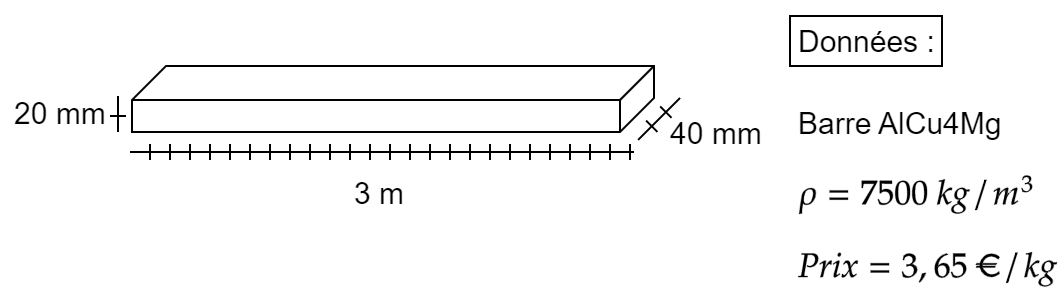
\includegraphics[scale=1]{Barre.png}


\marginnote{0,25 pt}
Réponse : 


%----------------------------------------------------------------------------------------

\end{document}